%%%%%%%%%%%%%%%%%%%%%%%%%%%%%%%%%%%%%%%%%
% Beamer Presentation
% LaTeX Template
% Version 1.0 (10/11/12)
%
% This template has been downloaded from:
% http://www.LaTeXTemplates.com
%
% License:
% CC BY-NC-SA 3.0 (http://creativecommons.org/licenses/by-nc-sa/3.0/)
%
%%%%%%%%%%%%%%%%%%%%%%%%%%%%%%%%%%%%%%%%%

%----------------------------------------------------------------------------------------
%	PACKAGES AND THEMES
%----------------------------------------------------------------------------------------

\documentclass{beamer}

\mode<presentation> {

\usetheme{Madrid}

\setbeamertemplate{navigation symbols}{} % To remove the navigation symbols from the bottom of all slides uncomment this line
}

\usepackage{graphicx} % Allows including images
\usepackage{booktabs} % Allows the use of \toprule, \midrule and \bottomrule in tables
\usepackage{amssymb}
\usepackage{amsmath}
\usepackage{textpos}
% \usepackage{subfigure}
\usepackage{cite}
\usepackage[T1]{fontenc}
\usepackage{subfig}
\usepackage{listings}

\definecolor{gray}{rgb}{0.4,0.4,0.4}
\definecolor{darkblue}{rgb}{0.0,0.0,0.6}
\definecolor{cyan}{rgb}{0.0,0.6,0.6}

\lstset{
  basicstyle=\ttfamily,
  columns=fullflexible,
  showstringspaces=false,
  commentstyle=\color{gray}\upshape
numbers=right, 
                numberstyle=\tiny, 
                breaklines=true,
                numbersep=5pt,
                xleftmargin=.25in,
                xrightmargin=.25in
}

\lstdefinelanguage{XML}
{
  morestring=[b]",
  morestring=[s]{>}{<},
  morecomment=[s]{<?}{?>},
  stringstyle=\color{black},
  identifierstyle=\color{darkblue},
  keywordstyle=\color{cyan},
  morekeywords={xmlns,version,type}% list your attributes here
}

\DeclareMathOperator*{\argmax}{\arg\!\max}

\title[Automatic Metadata Extraction]{Automatic Metadata Extraction \\ The High Energy Physics Use Case} % The short title appears at the bottom of every slide, the full title is only on the title page

\author{Joseph Boyd} % Your name
\institute[EPFL] % Your institution as it will appear on the bottom of every slide, may be shorthand to save space
{
\'Ecole Polytechnique F\'ed\'erale de Lausanne \\ % Your institution for the title page
\medskip
\textit{joseph.boyd@epfl.ch} % Your email address
}
\date{\today} % Date, can be changed to a custom date

\begin{document}

\begin{frame}
\titlepage % Print the title page as the first slide
\end{frame}

%------------------------------------------------

\section{Introduction}

%------------------------------------------------

\begin{frame}
\frametitle{Motivation}
\end{frame}

%------------------------------------------------

\begin{frame}
\frametitle{Aims}
\end{frame}

%------------------------------------------------

\section{Theory}

%------------------------------------------------

\begin{frame}[noframenumbering]{Outline}
\tableofcontents[currentsection, currentsubsection]
\end{frame}

%------------------------------------------------

\begin{frame}
\frametitle{Why CRFs?}
\end{frame}

%------------------------------------------------

\begin{frame}
\frametitle{Mathematical Formulation}
\end{frame}

%------------------------------------------------

\begin{frame}
\frametitle{Solution Approach}
\end{frame}

%------------------------------------------------

\section{Automatic Metadata Extraction}

%------------------------------------------------

\begin{frame}[noframenumbering]{Outline}
\tableofcontents[currentsection, currentsubsection]
\end{frame}

%------------------------------------------------

\begin{frame}
\frametitle{Metadata Extraction}
\end{frame}

%------------------------------------------------

\begin{frame}
\frametitle{GROBID}
\end{frame}

%------------------------------------------------

\begin{frame}
\frametitle{GROBID - CRF Cascade}
\begin{figure}[h]
\center
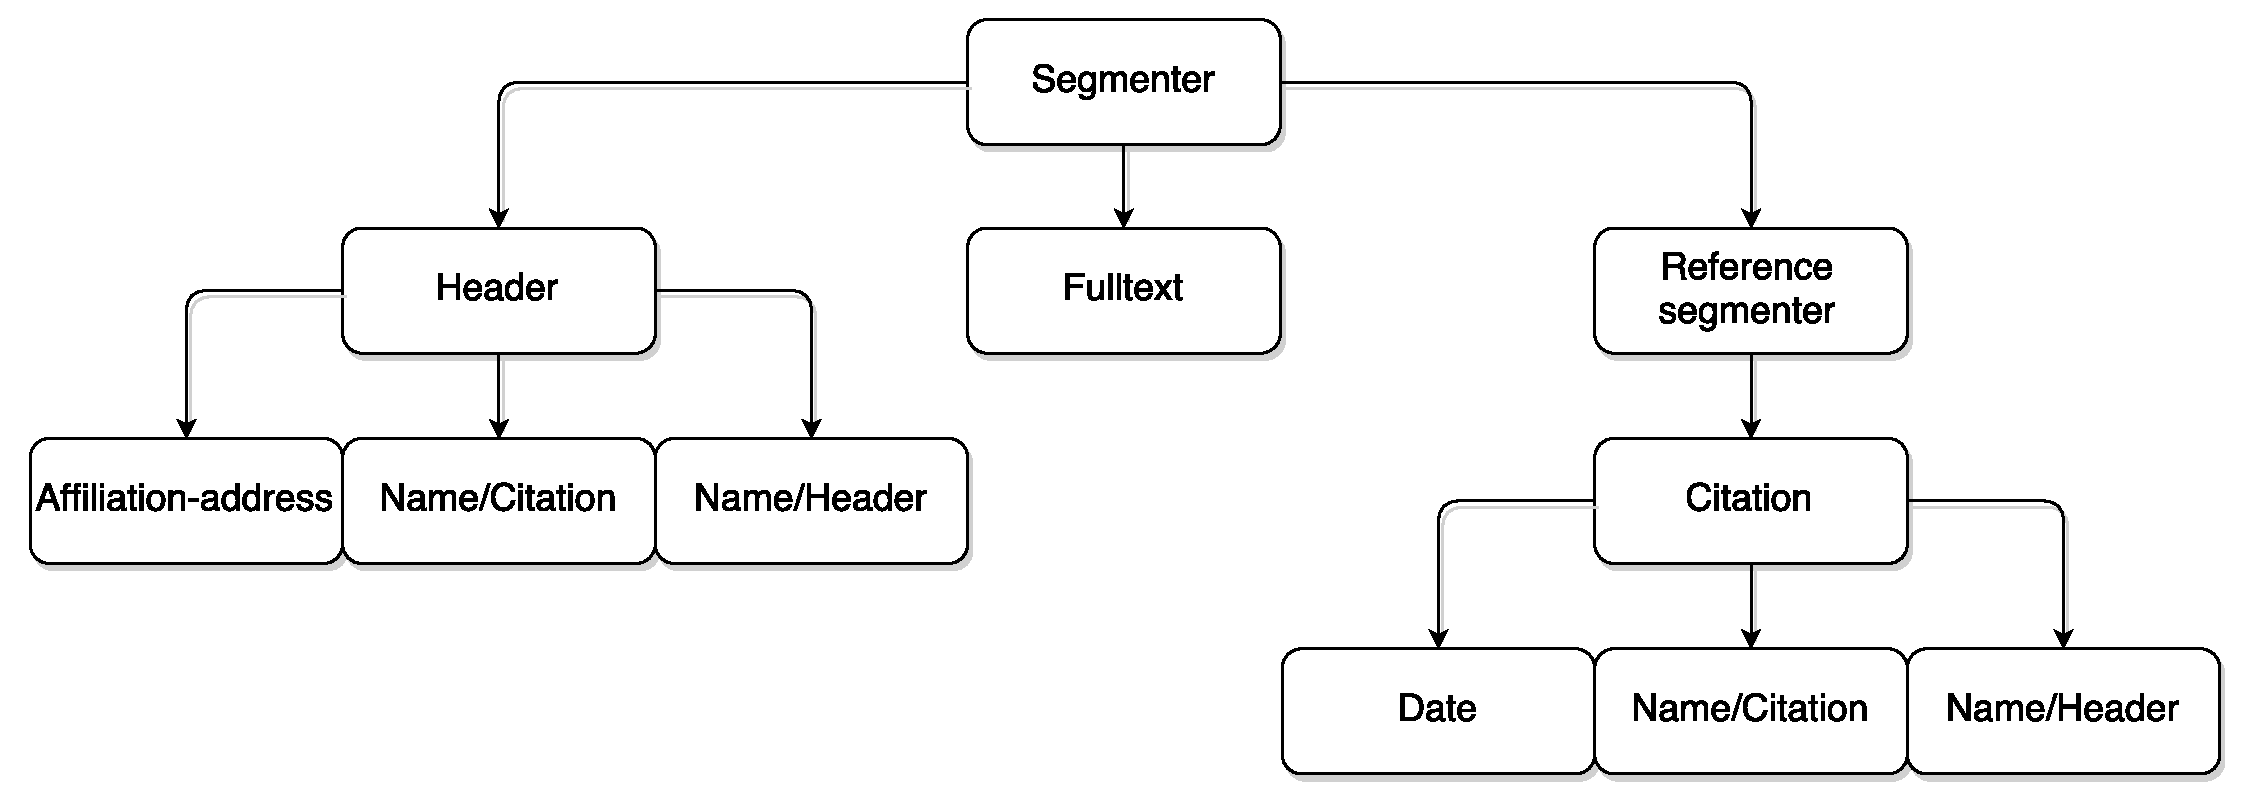
\includegraphics[width=4in]{Figures/cascade.pdf}
\caption{Cascade of models used by Grobid}
\end{figure}
\end{frame}

%------------------------------------------------

\section{Data, Methods, and Implementation}

%------------------------------------------------

\begin{frame}[noframenumbering]{Outline}
\tableofcontents[currentsection, currentsubsection]
\end{frame}

%------------------------------------------------

\begin{frame}
\frametitle{}
\begin{figure}[h]
\centering
\begin{tabular}{cc}
\subfloat[Collaboration field in header section.]{
\includegraphics[width=0.45\textwidth]{Figures/collaboration.pdf}}\label{fig:articlesamplesA}&
\subfloat[Discontinuous header data.]{
\includegraphics[width=0.45\textwidth]{Figures/eamonn.pdf}} \\
\subfloat[Collaboration author list.]{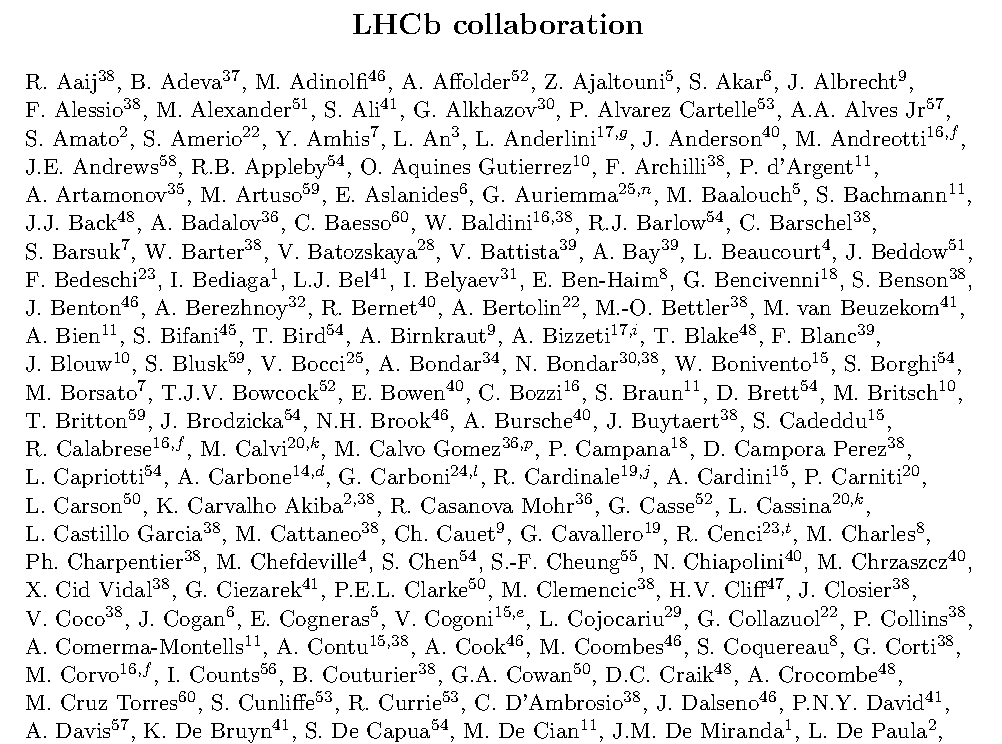
\includegraphics[width=0.45\textwidth]{Figures/authors.pdf}} & 
\subfloat[Collaboration affiliation list.]{
\includegraphics[width=0.45\textwidth]{Figures/affiliations.pdf}}\\
\end{tabular}
\caption{Figure (A) shows a collaboration field in a header section. Figure (B) shows discontinuous front matter that sits on the first page, but apart from the main header section and within the introductory section. Figures (C) and (D) give the authors list and affiliations for a large HEP collaboration; the author list begins on page 8 and continues to page 33. Figure (B) from (\cite{maguire2012taxonomy}), other excerpts from (\cite{aaij2015identification}).}
\label{fig:articlesamples}
\end{figure}
\end{frame}

%------------------------------------------------

\begin{frame}
\frametitle{}
\begin{table}[h]
\begin{center}
\begin{tabular}{|c|c|c|}
\hline
Model & HEP & CORA \\
\hline
Header & 157 papers & \textbf{2506 papers} \\
\hline
Segmentation & \textbf{169 papers} & 125 papers \\
\hline
\end{tabular}
\caption[Number of training instances for each model from each dataset.]{Number of training instances for each model from each dataset.}
\label{table:hepvscora}
\end{center}
\end{table}
\end{frame}

%------------------------------------------------

\begin{frame}
\frametitle{}
\end{frame}

%------------------------------------------------

\section{Key Results}

%------------------------------------------------

\begin{frame}[noframenumbering]{Outline}
\tableofcontents[currentsection, currentsubsection]
\end{frame}

%------------------------------------------------

\begin{frame}
\frametitle{}
\begin{figure}[h]
\center
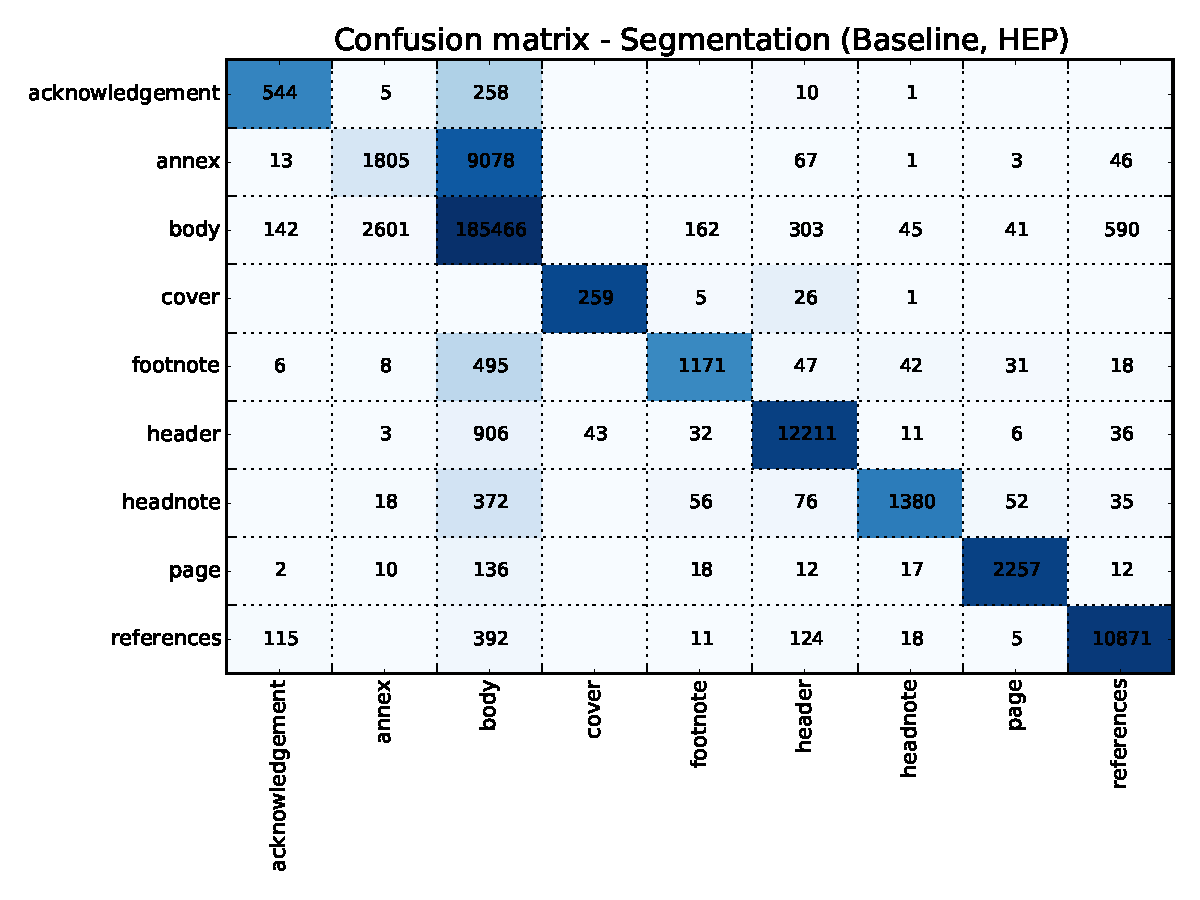
\includegraphics[width=4in]{Figures/baseline_confusion_segmentation.pdf}
\caption{Baseline confusion segmentation}
\end{figure}
\end{frame}

%------------------------------------------------

\begin{frame}
\frametitle{}
\begin{figure}[h]
\center
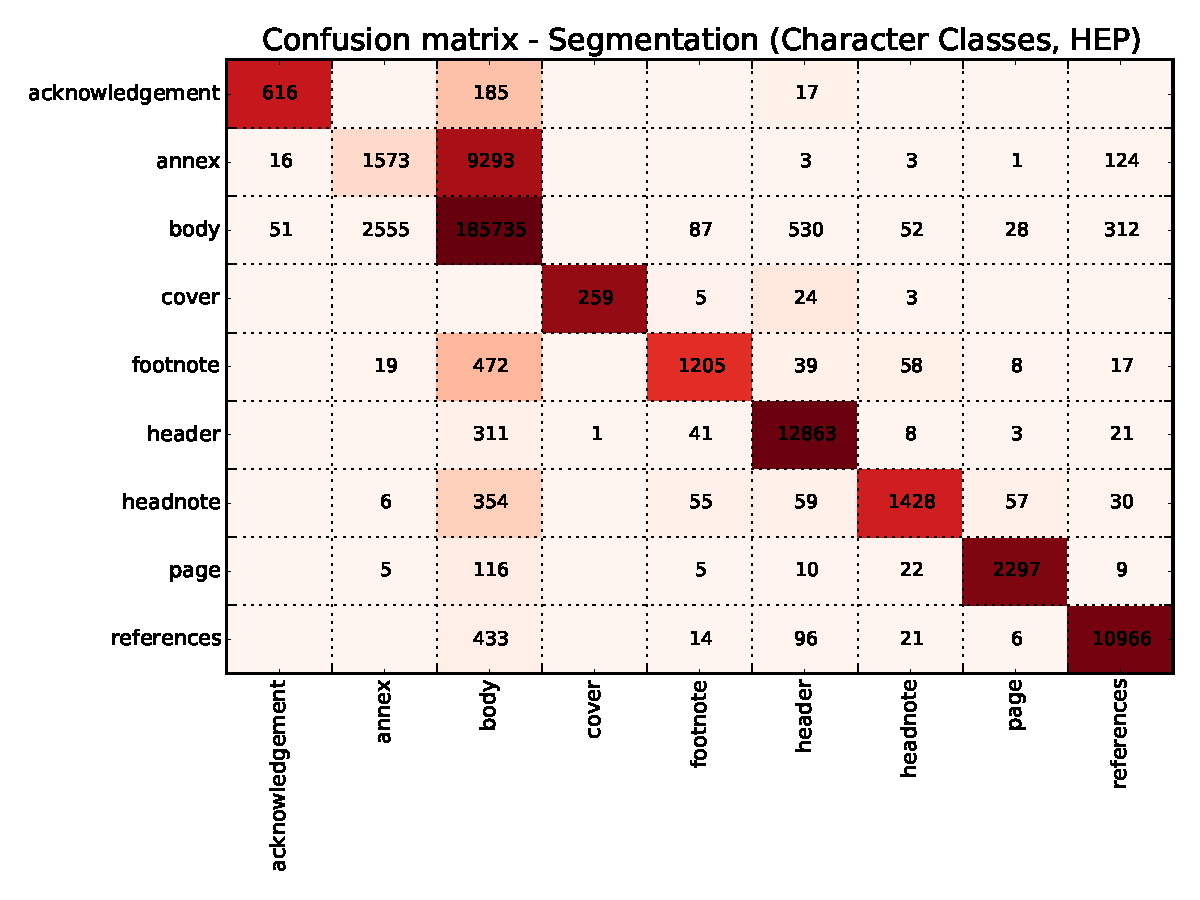
\includegraphics[width=4in]{Figures/classes_confusion_segmentation.pdf}
\caption{Classes confusion segmentation}
\end{figure}
\end{frame}

%------------------------------------------------

\begin{frame}
\frametitle{}
\end{frame}

%------------------------------------------------

\section{Conclusions}

%------------------------------------------------

\begin{frame}[noframenumbering]{Outline}
\tableofcontents[currentsection, currentsubsection]
\end{frame}

%------------------------------------------------

\begin{frame}
\frametitle{}
\end{frame}

%------------------------------------------------

\end{document} 